%% 08-experiments
\section{Experiments}
\label{sec:experiments}

All experiments are analytic or statevector simulations on CPU, using NumPy and
scikit-learn, and each completes in seconds to minutes. Seeds, resolved configurations
and library versions are recorded alongside every run. Every number quoted below is
generated from the experiment outputs rather than transcribed by hand.

\subsection{Setup}
\label{subsec:setup}

\paragraph{Datasets.}
We use WordNet nouns via NLTK, the molecular-function namespace of the Gene Ontology,
the Mammalia clade of the NCBI taxonomy, and synthetic regular $p$-ary trees for
controlled ablations. \Cref{tab:datasets} gives the shapes.

\begin{table}
  \centering
  \caption{The four hierarchies after preprocessing. Source columns describe the full
    reduced tree; the remaining columns describe the sample the kernels are evaluated
    on. Qubits is $\lceil \log_2 \abs{V} \rceil$ for the path-state encoding.}
  \label{tab:datasets}
  \small
  % Generated by code/experiments/collect_numbers.py -- do not edit.
\begin{tabular}{lrrrrrr}
\toprule
dataset & source nodes & source height & sampled leaves & nodes & radix & qubits \\
\midrule
synthetic $2$-ary & $511$ & $8$ & $256$ & $511$ & $2$ & $9$ \\
WordNet & $74\,374$ & $19$ & $256$ & $1\,028$ & $11$ & $11$ \\
Gene Ontology & $10\,041$ & $12$ & $256$ & $1\,235$ & $16$ & $11$ \\
NCBI Mammalia & $14\,722$ & $14$ & $256$ & $633$ & $38$ & $10$ \\
\bottomrule
\end{tabular}

\end{table}

\paragraph{Preprocessing, stated rather than assumed.}
Each of these sources is a directed acyclic graph in the wild, not a tree: WordNet
synsets can have several hypernyms. We reduce each to a tree by keeping, for every
node, the \emph{longest} path to the root, breaking ties by lexicographically smallest
identifier. Multiple inheritance is therefore discarded, which we record as a
limitation in \Cref{sec:limitations} rather than as a detail.

We then truncate every hierarchy at depth $\EOneHeight$. This is needed because the
$2^{\text{height}}$-dimensional product baselines are otherwise not representable:
WordNet reaches depth $\EOneSourceHeight$, so an angle or ZZ encoding would require
$2^{\EOneSourceHeight}$ amplitudes per point. Truncation also has the further benefit that
every encoding is compared on exactly the same tree. Finally we sample $\EOneLeaves$ leaves,
restrict to their ancestor closure, and pad shallow leaves to uniform depth. None of
these steps changes the lowest-common-ancestor depths among the sampled leaves below
the truncation, which is all the kernel depends on.

\paragraph{Baselines.}
Angle encoding, computational-basis encoding, a ZZ/IQP feature map with two
repetitions, a random product map, a block-product map where representable, and two
classical references: an RBF kernel on integer leaf coordinates and one on a one-hot
encoding. The geometric profile uses base $2$ throughout for the real datasets. Tying
the profile base to the branching factor instead, $\NCBIRadix$ for NCBI, pushes
$f(0)$ to around $10^{-13}$, below any resolution tolerance that a realistic shot
budget could support, so the base is treated as the free design parameter it is.

\subsection{E1: ultrametricity and resolution}
\label{subsec:e1}

\Cref{tab:e1} reports both diagnostics of \Cref{def:diagnostics} across all four
hierarchies, and \Cref{fig:e1-violations} plots them for WordNet.

\begin{table}
  \centering
  \caption{E1. Violation rate counts triples breaking \cref{eq:strong-triangle}; level
    constancy is zero exactly when the kernel is ultrametric with some profile;
    resolution is the number of distinguishable kernel values against the number of
    lowest-common-ancestor levels the sample populates. Only the path state scores well
    on both.}
  \label{tab:e1}
  \small
  % Generated by code/experiments/collect_numbers.py -- do not edit.
\begin{tabular}{llrrr}
\toprule
dataset & encoding & violation rate & level constancy & resolution \\
\midrule
synthetic $2$-ary & \textbf{path state (ours)} & $0$ & $0$ & 9 / 9 \\
 & basis & $0$ & $0$ & 2 / 9 \\
 & angle & $0.234$ & $0.496$ & 9 / 9 \\
 & ZZ / IQP & $0.275$ & $0.983$ & 9 / 9 \\
 & random product & $0.329$ & $0.927$ & 9 / 9 \\
\addlinespace
WordNet & \textbf{path state (ours)} & $0$ & $4.44 \times 10^{-16}$ & 9 / 9 \\
 & basis & $0$ & $0$ & 2 / 9 \\
 & angle & $0.322$ & $0.978$ & 9 / 9 \\
 & ZZ / IQP & $0.328$ & $0.48$ & 9 / 9 \\
 & random product & $0.329$ & $0.991$ & 9 / 9 \\
\addlinespace
Gene Ontology & \textbf{path state (ours)} & $0$ & $4.44 \times 10^{-16}$ & 9 / 9 \\
 & basis & $0$ & $0$ & 2 / 9 \\
 & angle & $0.322$ & $0.986$ & 9 / 9 \\
 & ZZ / IQP & $0.327$ & $0.748$ & 9 / 9 \\
 & random product & $0.329$ & $0.992$ & 9 / 9 \\
\addlinespace
NCBI Mammalia & \textbf{path state (ours)} & $0$ & $4.44 \times 10^{-16}$ & 9 / 9 \\
 & basis & $0$ & $0$ & 2 / 9 \\
 & angle & $0.323$ & $0.998$ & 9 / 9 \\
 & ZZ / IQP & $0.328$ & $0.605$ & 9 / 9 \\
 & random product & $0.329$ & $0.999$ & 9 / 9 \\
\addlinespace
\bottomrule
\end{tabular}

\end{table}

\begin{figure}
  \centering
  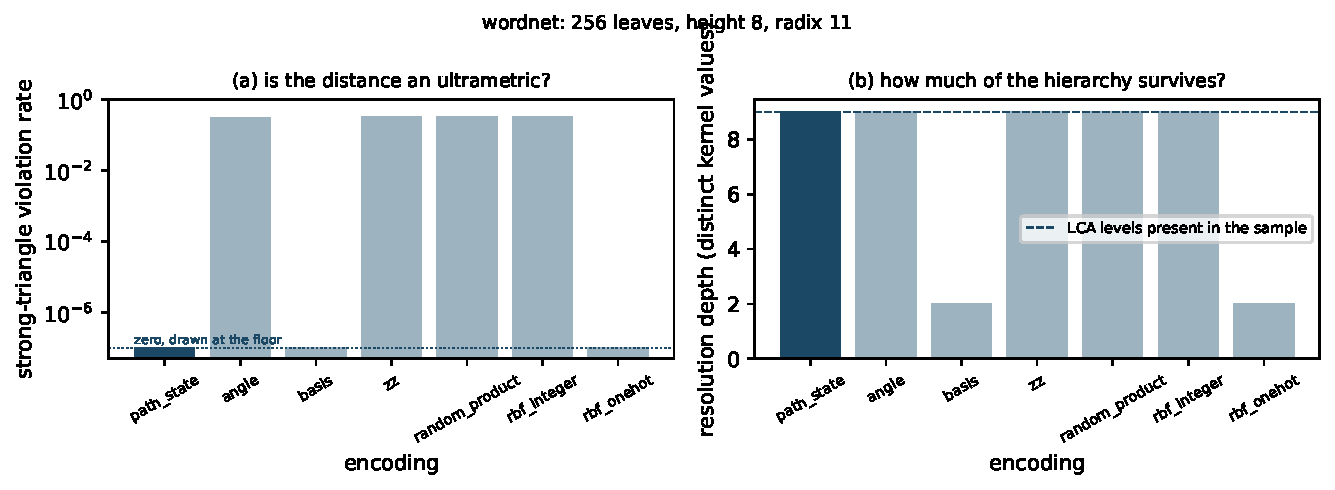
\includegraphics[width=\linewidth]{figures/e1_violations}
  \caption{E1 on WordNet. Panel~(a) asks whether the induced distance is an ultrametric
    at all; panel~(b) asks how much of the hierarchy survives. Basis encoding passes
    (a) perfectly and fails (b) completely, which is why both are reported.}
  \label{fig:e1-violations}
\end{figure}

Three readings. First, the path-state encoding attains level constancy
$\PathLevelConstancy$ and zero violations on every dataset, with full resolution: the
construction is exact on real hierarchies, not only on the regular trees of
\Cref{thm:path-states}. Second, every product and entangling baseline has a level
constancy near $1$: angle reaches $\AngleLevelConstancy$ and the random product map
$\RandProdLevelConstancy$. Their kernels are not merely imperfect ultrametrics
but are not ultrametric at all, in agreement with \Cref{thm:product-nogo,thm:dimension-bound}.

Third, and worth stating plainly because it complicates the headline: \textbf{basis
encoding also achieves zero violations}, with level constancy exactly zero. Its
resolution is $\BasisResolution$ out of $\EOneLevels$. This is the degenerate corner of
\Cref{thm:product-nogo} discussed in \Cref{sec:theorem-a}, and it is the reason we do
not claim that the path state is the unique encoding with an ultrametric kernel. The
correct claim is narrower and, we think, more useful: it is the only one that is both
ultrametric and fully resolving.

\subsection{E2: hierarchical classification}
\label{subsec:e2}

\Cref{tab:e2} reports five-fold cross-validated accuracy for predicting a leaf's
depth-$2$ ancestor, together with the Spearman correlation between the kernel's induced
distance and true tree distance. Classes with fewer than five members are dropped and
the count is reported in the run metadata; no hyperparameter was tuned.

\begin{table}
  \centering
  \caption{E2. Accuracy is five-fold cross-validated with a precomputed-kernel SVM at
    $C = 1$. A dash marks an undefined rank correlation: a delta kernel assigns every
    distinct pair the same distance, so no correlation exists.}
  \label{tab:e2}
  \small
  % Generated by code/experiments/collect_numbers.py -- do not edit.
\begin{tabular}{lrrrrrr}
\toprule
encoding & \multicolumn{2}{c}{WordNet} & \multicolumn{2}{c}{Gene Ontology} & \multicolumn{2}{c}{NCBI Mammalia} \\
\cmidrule(lr){2-3}\cmidrule(lr){4-5}\cmidrule(lr){6-7}
& acc. & $\rho$ & acc. & $\rho$ & acc. & $\rho$ \\
\midrule
\textbf{path state (ours)} & $0.79$ & $1$ & $0.6$ & $1$ & $1$ & $1$ \\
angle & $0.67$ & $0.17$ & $0.56$ & $0.13$ & $0.85$ & $-0.006$ \\
ZZ / IQP & $0.48$ & $0.098$ & $0.48$ & $0.16$ & $0.9$ & $0.1$ \\
random product & $0.84$ & $0.37$ & $0.75$ & $0.28$ & $1$ & $0.35$ \\
basis & $0.21$ & --- & $0.28$ & --- & $0.68$ & --- \\
RBF (integer) & $0.15$ & $0.0037$ & $0.27$ & $0.027$ & $0.68$ & $0.064$ \\
\bottomrule
\end{tabular}

\end{table}

The path state attains $\rho = \ETwoPathRho$ on every dataset. This is not a fitted
result and should not be read as one: by \cref{eq:exactness} the induced distance is a
strictly monotone function of tree distance, so perfect rank correlation is a
consequence of the construction. No baseline exceeds $\ETwoBestBaselineRho$.

On accuracy the picture is different, and we report it as it came out. On WordNet the
path state reaches $\ETwoPathAccuracy \pm \ETwoPathAccuracyStd$ while the
\ETwoBestBaseline{} baseline reaches $\ETwoBestBaselineAccuracy$; the ordering is
similar on Gene Ontology. A kernel that faithfully encodes tree distance is therefore
\emph{not} the best kernel for this classification task, which is unsurprising once
stated: the label is the depth-$2$ ancestor, and a kernel that also spends
representational capacity on depths $3$ through $\EOneHeight$ is spending it on distinctions the
label ignores. Geometric fidelity and task accuracy are different objectives, and this
paper claims the former.

The comparison against v-PuNNs \citep{Nguessan2025VPuNNs}, which reports $99.96\%$ leaf
accuracy on WordNet, must be read the same way and is not close. That is a trained deep
model with a bespoke optimiser over $p$-adic weight space; this is a fixed encoding
with a closed form and no parameters. We record the gap rather than reframing it: on
accuracy, the trained model wins by a wide margin. The criterion for this experiment
was fixed before any number was produced, precisely so that a weak result could not
tempt a retrofit of the paper's claims.

\subsection{E3: ablations}
\label{subsec:e3}

\Cref{fig:e3-ablation} sweeps the profile shape, tree depth and branching factor over
$\EThreeConfigs$ configurations.

\begin{figure}
  \centering
  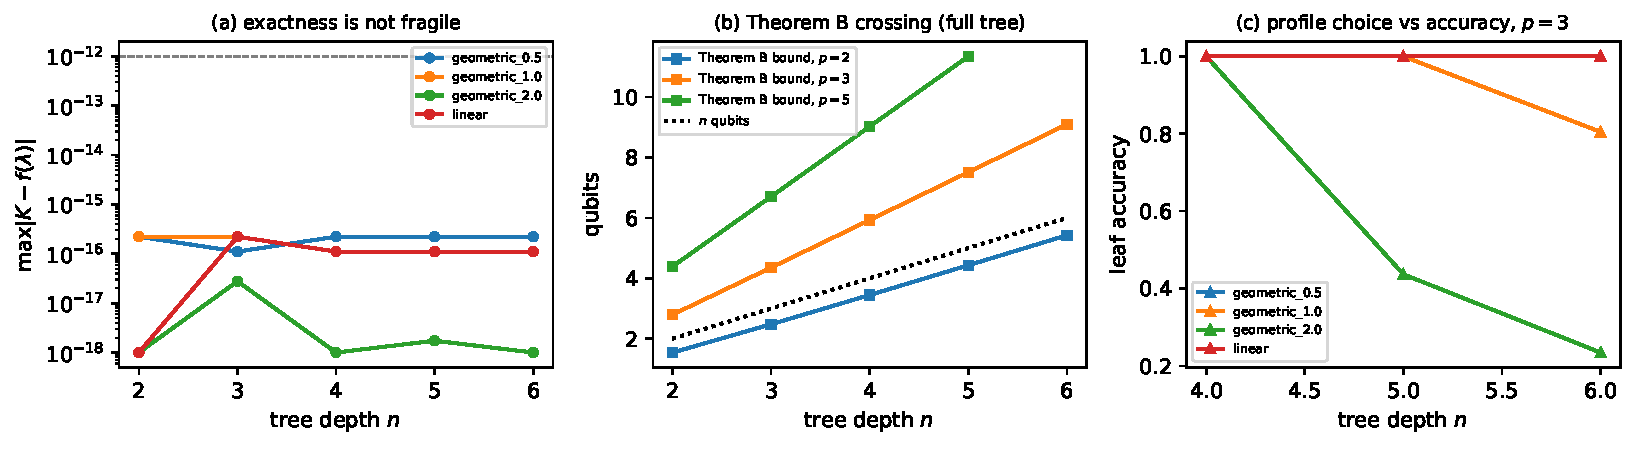
\includegraphics[width=\linewidth]{figures/e3_ablation}
  \caption{E3. (a) The profile residual stays at machine precision for every strictly
    monotone profile at every depth. (b) The \Cref{thm:dimension-bound} bound against
    the $n$ qubits a product or IQP encoding provides: above the diagonal for
    $p \ge 3$, below it for $p = 2$. (c) Profile choice against accuracy.}
  \label{fig:e3-ablation}
\end{figure}

Panel~(a) is the robustness check for \Cref{thm:path-states}: the worst residual over
all $\EThreeConfigs$ configurations is $\EThreeWorstResidual$, and the total number of
strong-triangle violations is $\EThreeMaxViolations$. Exactness does not degrade with
depth, radix or profile shape.

Panel~(b) is the picture of \Cref{cor:no-n-qubit}. For $p = 3$ and $p = 5$ the required
qubit count runs above the diagonal at every depth, so no $n$-qubit encoding can
realise the kernel. For $p = 2$ it runs below, which is \Cref{rem:complementarity}: at
radix two the dimension bound alone is not enough and \Cref{thm:product-nogo} carries
the argument. The curves use the closed form \cref{eq:row-sum} on the full tree, since
an estimate from a subsample saturates at $\log_2$ of the sample size.

\subsection{E4: the re-uploading trade-off}
\label{subsec:e4}

\begin{figure}
  \centering
  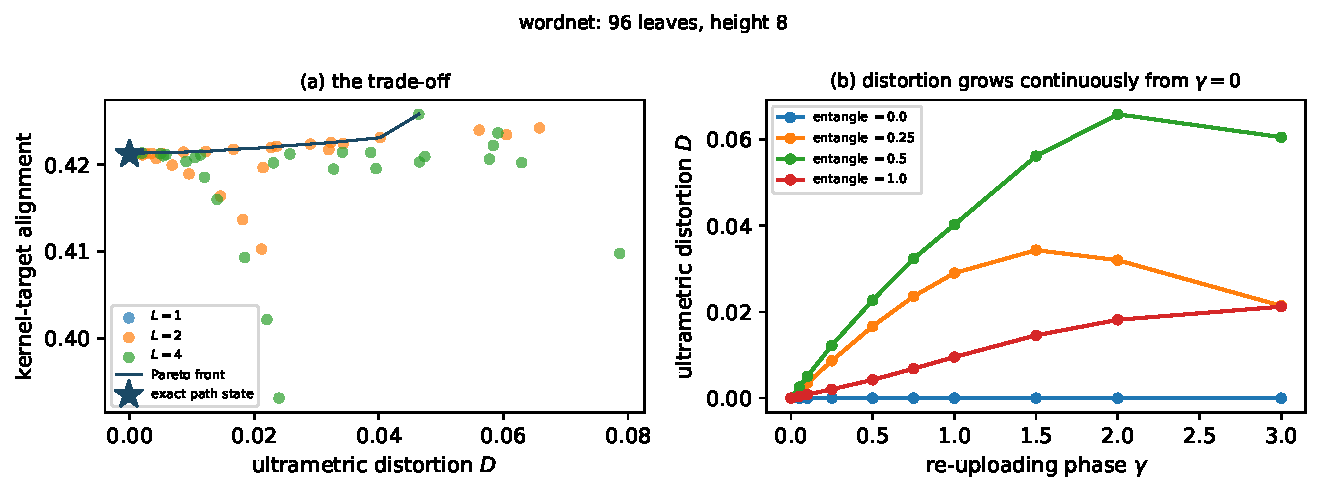
\includegraphics[width=\linewidth]{figures/e4_pareto}
  \caption{E4 on WordNet, over $\EFourConfigs$ configurations of the family
    \cref{eq:reupload}. Distortion grows continuously from zero, so the exact
    construction is the endpoint of a tunable family rather than an isolated point ---
    but the alignment available in exchange is small.}
  \label{fig:e4-pareto}
\end{figure}

Distortion grows continuously from zero as the re-uploading phase increases, which
answers the structural question: the exact construction is not an isolated special
case but the zero-distortion endpoint of a continuum. The quantitative answer is less
encouraging. The exact point achieves alignment $\EFourExactAlignment$, and the best
configuration anywhere in the family achieves $\EFourBestAlignment$ at distortion
$\EFourBestDistortion$, a gain of $\EFourAlignmentGain$. On these datasets the
trade-off exists but buys very little, and we would not recommend paying for it.

\subsection{E5: noise and finite shots}
\label{subsec:e5}

\begin{figure}
  \centering
  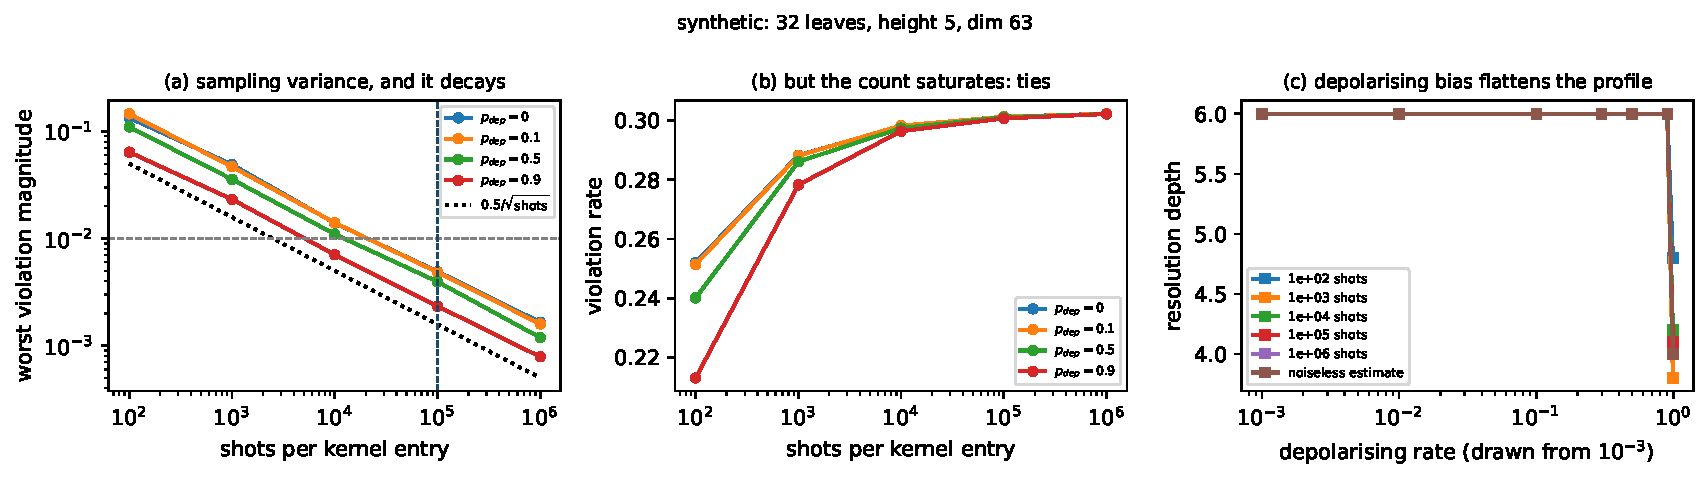
\includegraphics[width=\linewidth]{figures/e5_noise}
  \caption{E5. (a) The violation magnitude decays as $O(1/\sqrt{\text{shots}})$,
    tracking the dotted reference line. (b) The violation \emph{count} saturates
    instead, because a constant fraction of triples in an ultrametric is exactly tight.
    (c) Depolarising noise leaves ultrametricity intact but flattens the profile until
    resolution collapses.}
  \label{fig:e5-noise}
\end{figure}

\Cref{prop:depolarising} predicts that depolarising noise cannot break ultrametricity,
and the measurement agrees exactly: at every rate up to $0.99$, the noiseless-estimate
row has zero violations and zero excess. What degrades is resolution, and only at
extreme rates.

Finite sampling is the real constraint, and measuring it correctly required abandoning
the obvious statistic. The violation count \emph{increases} with the shot budget,
rising towards a plateau, which looks like a bug and is not: $\TieFraction$ of triples
in this ultrametric meet \cref{eq:strong-triangle} with equality, and any perturbation
flips about half of them, so the count converges to that tie fraction rather than to
zero. The violation magnitude behaves as expected, falling from $\ExcessAtLowShots$ at
$\ExcessAtLowShotsCount$ shots to $\ExcessAtHighShots$ at $\ExcessAtHighShotsCount$
shots, a factor of $\sqrt{10}$ per decade. Defining the budget on the magnitude gives
\textbf{$\ShotBudget$ shots per kernel entry} for a worst-case excess below
$\ShotTargetExcess$, over $\ENoiseRepeats$ repetitions.
